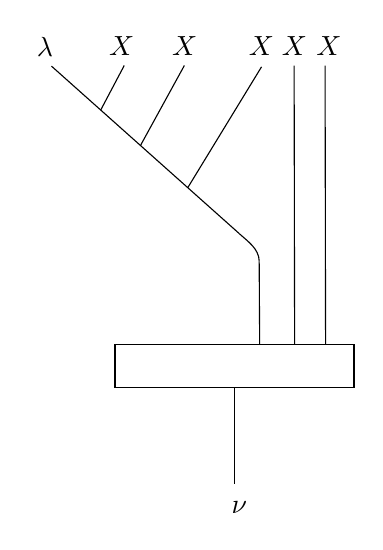
\begin{tikzpicture}[yscale=-1,scale=0.03,baseline={([yshift=-.5ex]current bounding box.center)}]
\begin{scope}[shift={(0.00mm,719.29mm)}]
% path id='path4136'
% path spec='m 321.64395,461.81069 0,180 1011.42855,0 0,-180 z'
\draw [fill=none,draw=black] (321.64mm,461.81mm)
-- ++(0.00mm,180.00mm)
-- ++(1011.43mm,0.00mm)
-- ++(0.00mm,-180.00mm)
-- cycle
;
% path id='path4138'
% path spec='m 827.14286,641.79073 0,410.57157'
\draw [fill=none,draw=black] (827.14mm,641.79mm)
-- ++(0.00mm,410.57mm)
;
% path id='path4140'
% path spec='M 933.94279,462.27605 931.8593,109.22944'
\draw [fill=none,draw=black] (933.94mm,462.28mm)
-- (931.86mm,109.23mm)
;
% path id='path4142'
% path spec='m 1081.8843,461.91167 -2.0829,-1181.11335'
\draw [fill=none,draw=black] (1081.88mm,461.91mm)
-- ++(-2.08mm,-1181.11mm)
;
% path id='path4144'
% path spec='m 1212.9521,461.91167 -2.083,-1181.11335'
\draw [fill=none,draw=black] (1212.95mm,461.91mm)
-- ++(-2.08mm,-1181.11mm)
;
% path id='path4204'
% path spec='M 931.96674,109.25855 C 931.27826,56.48405 884.0324,25.300792 847.99781,-7.41407'
\draw [fill=none,draw=black] (931.97mm,109.26mm)
%%%% Warning: check controls
.. controls (931.28mm,56.48mm) and (884.03mm,25.30mm) .. (848.00mm,-7.41mm)
;
% path id='path4206'
% path spec='M 848.25,-7.32528 52.500093,-716.9502'
\draw [fill=none,draw=black] (848.25mm,-7.33mm)
-- (52.50mm,-716.95mm)
;
% path id='path4208'
% path spec='m 360.62446,-719.64737 -99.56947,188.48815'
\draw [fill=none,draw=black] (360.62mm,-719.65mm)
-- ++(-99.57mm,188.49mm)
;
% path id='path4210'
% path spec='M 615.1829,-719.64737 429.29592,-380.90033'
\draw [fill=none,draw=black] (615.18mm,-719.65mm)
-- (429.30mm,-380.90mm)
;
% path id='path4212'
% path spec='m 941.86623,-713.99052 -312.4307,511.79063'
\draw [fill=none,draw=black] (941.87mm,-713.99mm)
-- ++(-312.43mm,511.79mm)
;
\node [black] at (848.00mm,1150mm) { $\nu$ };
\node [black] at (25.00mm,-800mm) { $\lambda$ };
\node [black] at (350.10mm,-800mm) { $X$ };
\node [black] at (616.43mm,-800mm) { $X$ };
\node [black] at (941.25mm,-800mm) { $X$ };
\node [black] at (1080.63mm,-800mm) { $X$ };
\node [black] at (1226.97mm,-800mm) { $X$ };
\end{scope}
\end{tikzpicture}
